\documentclass{article}
\usepackage{graphicx}
\graphicspath{{images/}}

\usepackage[english]{babel}
\usepackage{biblatex}
\addbibresource{references.bib}


\title{Simple LaTeX document!}
\author{Teemu Koivumaa}
\date{20 November 2022}

\begin{document}
\maketitle
\thispagestyle{empty}

\newpage
\tableofcontents
\thispagestyle{empty}

\newpage
\pagenumbering{arabic} 
\section{Maths}
\subsection{Pythagorean theorem}
In pythagorean equation (as seen below) \textbf{a} and \textbf{b} represent lengths of a triangle’s two sides and \textbf{c} the lenght of the hypotenuse.

\begin{equation}
a^2 + b^2 = c^2
\end{equation}

\subsection{Function}
This is a simple math function.
\begin{equation}
f(x) = x^2
\end{equation}

\section{Figure}
This is a figure\ref{fig:figure} of the math function.
\\
\\
\begin{figure}[h]
    \centering
    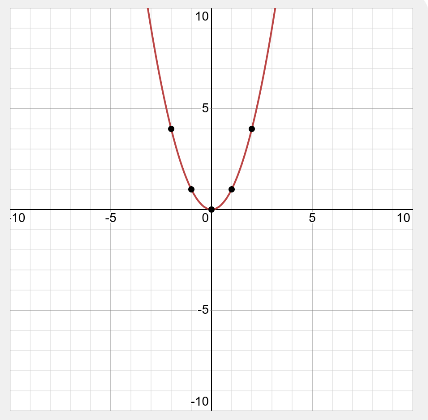
\includegraphics[scale=0.25]{FunctionGraph.png}
    \caption{A figure of the math function \cite{algebra_examples_2022}}
    \label{fig:figure}
\end{figure}


\section{Table}
This table\ref{table:data} contains important information.
\begin{table}[h!]
\centering
\begin{tabular}{|l|l|}
\hline
Important thing & Relativity \\ \hline
5050            & 50\%       \\ \hline
325             & 23\%       \\ \hline
432             & 99\%       \\ \hline
\end{tabular}
\caption{Table that contains important information}
\label{table:data}
\end{table}

\newpage
\section{Referencing}
\printbibliography

\end{document}
